% Intended LaTeX compiler: pdflatex
\documentclass[10pt,a4paper,UTF8]{article}
\usepackage{zclorg}
\usepackage{tikztheorem}
\author{zcl.space}
\date{}
\title{超几何分布}
\hypersetup{
 pdfauthor={zcl.space},
 pdftitle={超几何分布},
 pdfkeywords={probability},
 pdfsubject={},
 pdfcreator={Emacs 25.0.50.1 (Org mode 9.0.6)},
 pdflang={English}}
\begin{document}

\maketitle
\tableofcontents
\titlepic{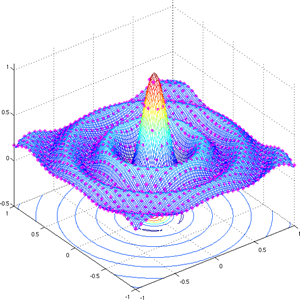
\includegraphics[scale=0.25]{../../img/sinc.PNG}}


\section{定义}
\label{sec:org853d906}


设一个坛子里一共有\(N\)个球,其中\(m\)个白球,\(N-m\)个黑球,从中随机的(无放回)取出\(n\)个球,令\(X\)表示取出来的白球数,那么:
\begin{equation}
\label{eq:1}
P\{X = i\} = \frac{\binom{m}{i} \binom{N-m}{n-i}}{\binom{N}{n}},\quad i = 0,1,\ldots ,n
\end{equation}

一个随机变量\(X\),如果其概率分布满足式 (\ref{eq:1})就说\(X\)服从超几何分布。
\section{超几何分布的期望和方差}
\label{sec:org98ac021}


我们采用和 \href{binary-distribution.org}{二项分布} 类似的计算方法。
\begin{eqnarray}
\label{eq:2}
E[X^{k}]&=& \sum_{i=0}^{n}i^{k}P\{X=i\} \\
&=& \sum_{i=1}^{n}i^{k}\binom{m}{i}\binom{N-m}{n-i}/\binom{N}{n}\\
&=&\frac{mn}{N}\sum_{i=1}^{n}i^{k-1}\binom{m-1}{i-1}\binom{N-m}{n-i}/\binom{N-1}{n-1}\\
&=&\frac{mn}{N}\sum_{j=0}^{n-1}(j+1)^{k-1}\frac{\binom{m-1}{j}\binom{N-m}{n-1-j}}{\binom{N-1}{n-1}}\\
&=& \frac{mn}{N}E[(Y+1)^{k-1}]
\end{eqnarray}

其中\(Y\)是参数为\((n-1,N-1,m-1)\)的超几何随机变量。在上式的求解过程中,我们用到了两个恒等式:
\begin{eqnarray}
\label{eq:3}
i\binom{m}{i}&=&m\binom{m-1}{i-1} \\
n\binom{N}{n}&=&N\binom{N-1}{n-1}
\end{eqnarray}

对于式 (\ref{eq:2}),我们令\(k=1\),所以有:
\begin{equation}
\label{eq:4}
E[X] = \binom{mn}{N}
\end{equation}
换句话说,如果从\(N\)个球(其中有\(m\)个白球)中随机抽取\(n\)个,那么其中白球数的期望为\(mn/N\)。

对于式 (\ref{eq:2}),令\(k=2\),则有:
\begin{eqnarray}
\label{eq:5}
E[X^{2}]&=& \frac{mn}{N}E[Y+1] \\
&=& \frac{mn}{N}\bigg[ \frac{(n-1)(m-1)}{N-1} + 1 \bigg]
\end{eqnarray}

另外\(E[X] = mn/N\),所以我们有:
\begin{equation}
\label{eq:6}
\mathrm{Var}(X) = \frac{mn}{N}\bigg[ \frac{(n-1)(m-1)}{N-1} + 1 - \frac{mn}{N}\bigg]
\end{equation}
令\(p=m/N\),并利用恒等式:
\begin{equation}
\label{eq:7}
\frac{m-1}{N-1} = \frac{Np-1}{N-1} = p - \frac{1-p}{N-1}
\end{equation}
得到:
\begin{equation}
\label{eq:8}
\mathrm{Var}(X) = np(1-p)(1-\tfrac{n-1}{N-1})
\end{equation}

对于超几何分布,我们知道期望为\(\frac{mn}{N} = np ,p = \frac{m}{N}\),\(p\)是白球的比例。当\(N\)很大时,观察 (\ref{eq:8}),我们有:
\begin{equation}
\label{eq:9}
\mathrm{Var}[X] \approx np(1-p)
\end{equation}

回忆二项分布,我们很容易发现其和超几何分布的相似性。
\section{例子}
\label{sec:orgeaac9eb}


栖息于某个地区的动物个体总数为\(N\),为了得到这个\(N\)的大致估计,神态学家常常做这样的试验:先捉住\(m\)个,然后打上标签,放回大自然。过一段时间,等这\(m\)个动物充分分散到其他动物中的时,再捕捉\(n\)个。假设\(X\)为第二批捕捉的\(n\)个动物中带标记的个数。如果前后两次捕捉过程中动物的总数没有发生变化,而且捉住每一只动物的可能性是一样的,那么\(X\)为一超几何随机变量,满足:
\begin{equation}
\label{eq:10}
P\{X = i\} = \frac{\binom{m}{i} \binom{N-m}{n-i}}{\binom{N}{n}} = P_{i}(N)
\end{equation}
现在假设\(i\)为\(X\)的观测值,那么因为\(P_{i}(N)\)表示该地区事实上总共有\(N\)个动物的条件下观测时间\(X\)的取值的概率,故使\(P_{i}(N)\)达到最大值的\(N\)值应当是动物个体总数\(N\)的一个合理估计。这样的估计称为极大似然估计估计。

求\(P_{i}(N)\)最大值的最简单的方法是:首先注意
\begin{equation}
\label{eq:11}
\frac{P_{i}(N)}{P_{i}(N-1)} = \frac{(N-m)(N-n)}{N(N-m-n+i)}
\end{equation}
使上式中的比值大于1,则有:
\begin{equation}
\label{eq:12}
(N-m)(N-n) \geq N(N-m-n+i)
\end{equation}
或者必须有:
\begin{equation}
\label{eq:13}
N \leq \frac{mn}{i}
\end{equation}
所以\(P_{i}(N)\)值是先上升然后下降。且在不超过\(mn/i\)的最大整数处达到其最大值。这个最大整数就是\(N\)的最大似然估计。

上述估计还可以这样求得:假设在这个地区内有标记的动物所占的比例为\(m/N\),应当近似的等于第二次捕捉的动物中做过标记的动物所占的比例\(i/n\)。
\section{超几何分布和二项分布的关系}
\label{sec:org5f1972c}


从\(N\)个球(白球比例为\(p = m/N\))中,无放回随机抽取\(n\)个球,那么取中的白球数为超几何分布随机变量。如果对于\(n\)来讲,\(m\)和\(N\)都很大,那么有放回和无放回取球没什么差别,因为当\(m\)和\(N\)很大时,不管前面取了哪个球,接下来的取到的失败求的概率任然近似于\(p\)。换言之,当\(m\)和\(N\)相比\(n\)很大时,\(X\)的分布列应该近似等于参数为\((n,p)\)的二项随机变量的分布列。为了证明这个直觉,注意,如果\(X\)是超几何分布,那么对于\(i\leq n\)有:
\begin{eqnarray}
\label{eq:15}
P\{X=i\}&=& \frac{\binom{m}{i}\binom{N-m}{n-i}}{\binom{N}{n}} \\
&=&\frac{m!}{(m-i)!i!}\frac{(N-m)!}{(N-m-n+i)!(n-i)!}\frac{(N-n)!n!}{N!}\\
&=&\binom{n}{i} \frac{m}{N}\frac{m-1}{N-1}\cdots\frac{m-i+1}{N-i+1}\frac{N-m}{N-i}\frac{N-m-1}{N-i-1}\cdots \frac{N-m-(n-i-1)}{N-i-(n-i-1)} \\
&=&\binom{n}{i}p^{i}(1-p)^{n-i}
\end{eqnarray}
其中最后一个等式成立的条件时\(p=m/N\)且\(m,N\)相对于\(n\)和\(i\)都很大。我们在求超几何变量的期望和方差时也验证了这个结论。
\end{document}
